\documentclass[12pt]{article}
\usepackage{graphicx} % Required for inserting images
\usepackage{biblatex}
\usepackage{hyperref}
\usepackage{fullpage}
\usepackage{listings}
\usepackage{xcolor}
\usepackage{amsmath}
\usepackage{amsfonts}

\bibliography{rust_model_checking}

\title{CS6110: Software Verification Final Project: Formal Verification of Rust Programs with Creusot}
\author{Taylor Allred \texttt{taylor.allred21@gmail.com}\\ Ashton Wiersdorf \texttt{research@wiersdorfmail.net}}
\date{Spring 2023}

\pagenumbering{gobble}
\begin{document}

\maketitle

\begin{abstract}
\noindent
Rust is the hottest new language in systems programming.
Its linear type system provides compile-time guarantees about memory resources and avoids race-conditions.
With an increased reliance on Rust for critical code, there's a greater need for verification tools.
Several new tools have popped up to fill this need: in particular, we are looking at Creusot, a formal verification system.
In our project, we learned about and tried verifying code with Creusot.
Our experience convinced us that the project seems very useful for verifying Rust code in theory but still needs some improvement for usability.
If nothing else, Creusot shows how to utilize Rust's unique features as well as existing theorem provers to make a compelling verification tool.
\end{abstract}

\setcounter{tocdepth}{2}
\tableofcontents

\clearpage
\pagenumbering{arabic}
\section{Overview of Creusot}

Creusot\cite{denisCreusot2023} is a tool for formally verifying Rust programs.
Creusot allows you to write specification for your software using Rust macros, and then defer to the Why3\cite{bobotWhy3ShepherdYour} platform to discharge those proofs.

Here is an overview of Creusot's role in verifying Rust software:

\begin{figure}[h]
  \centering
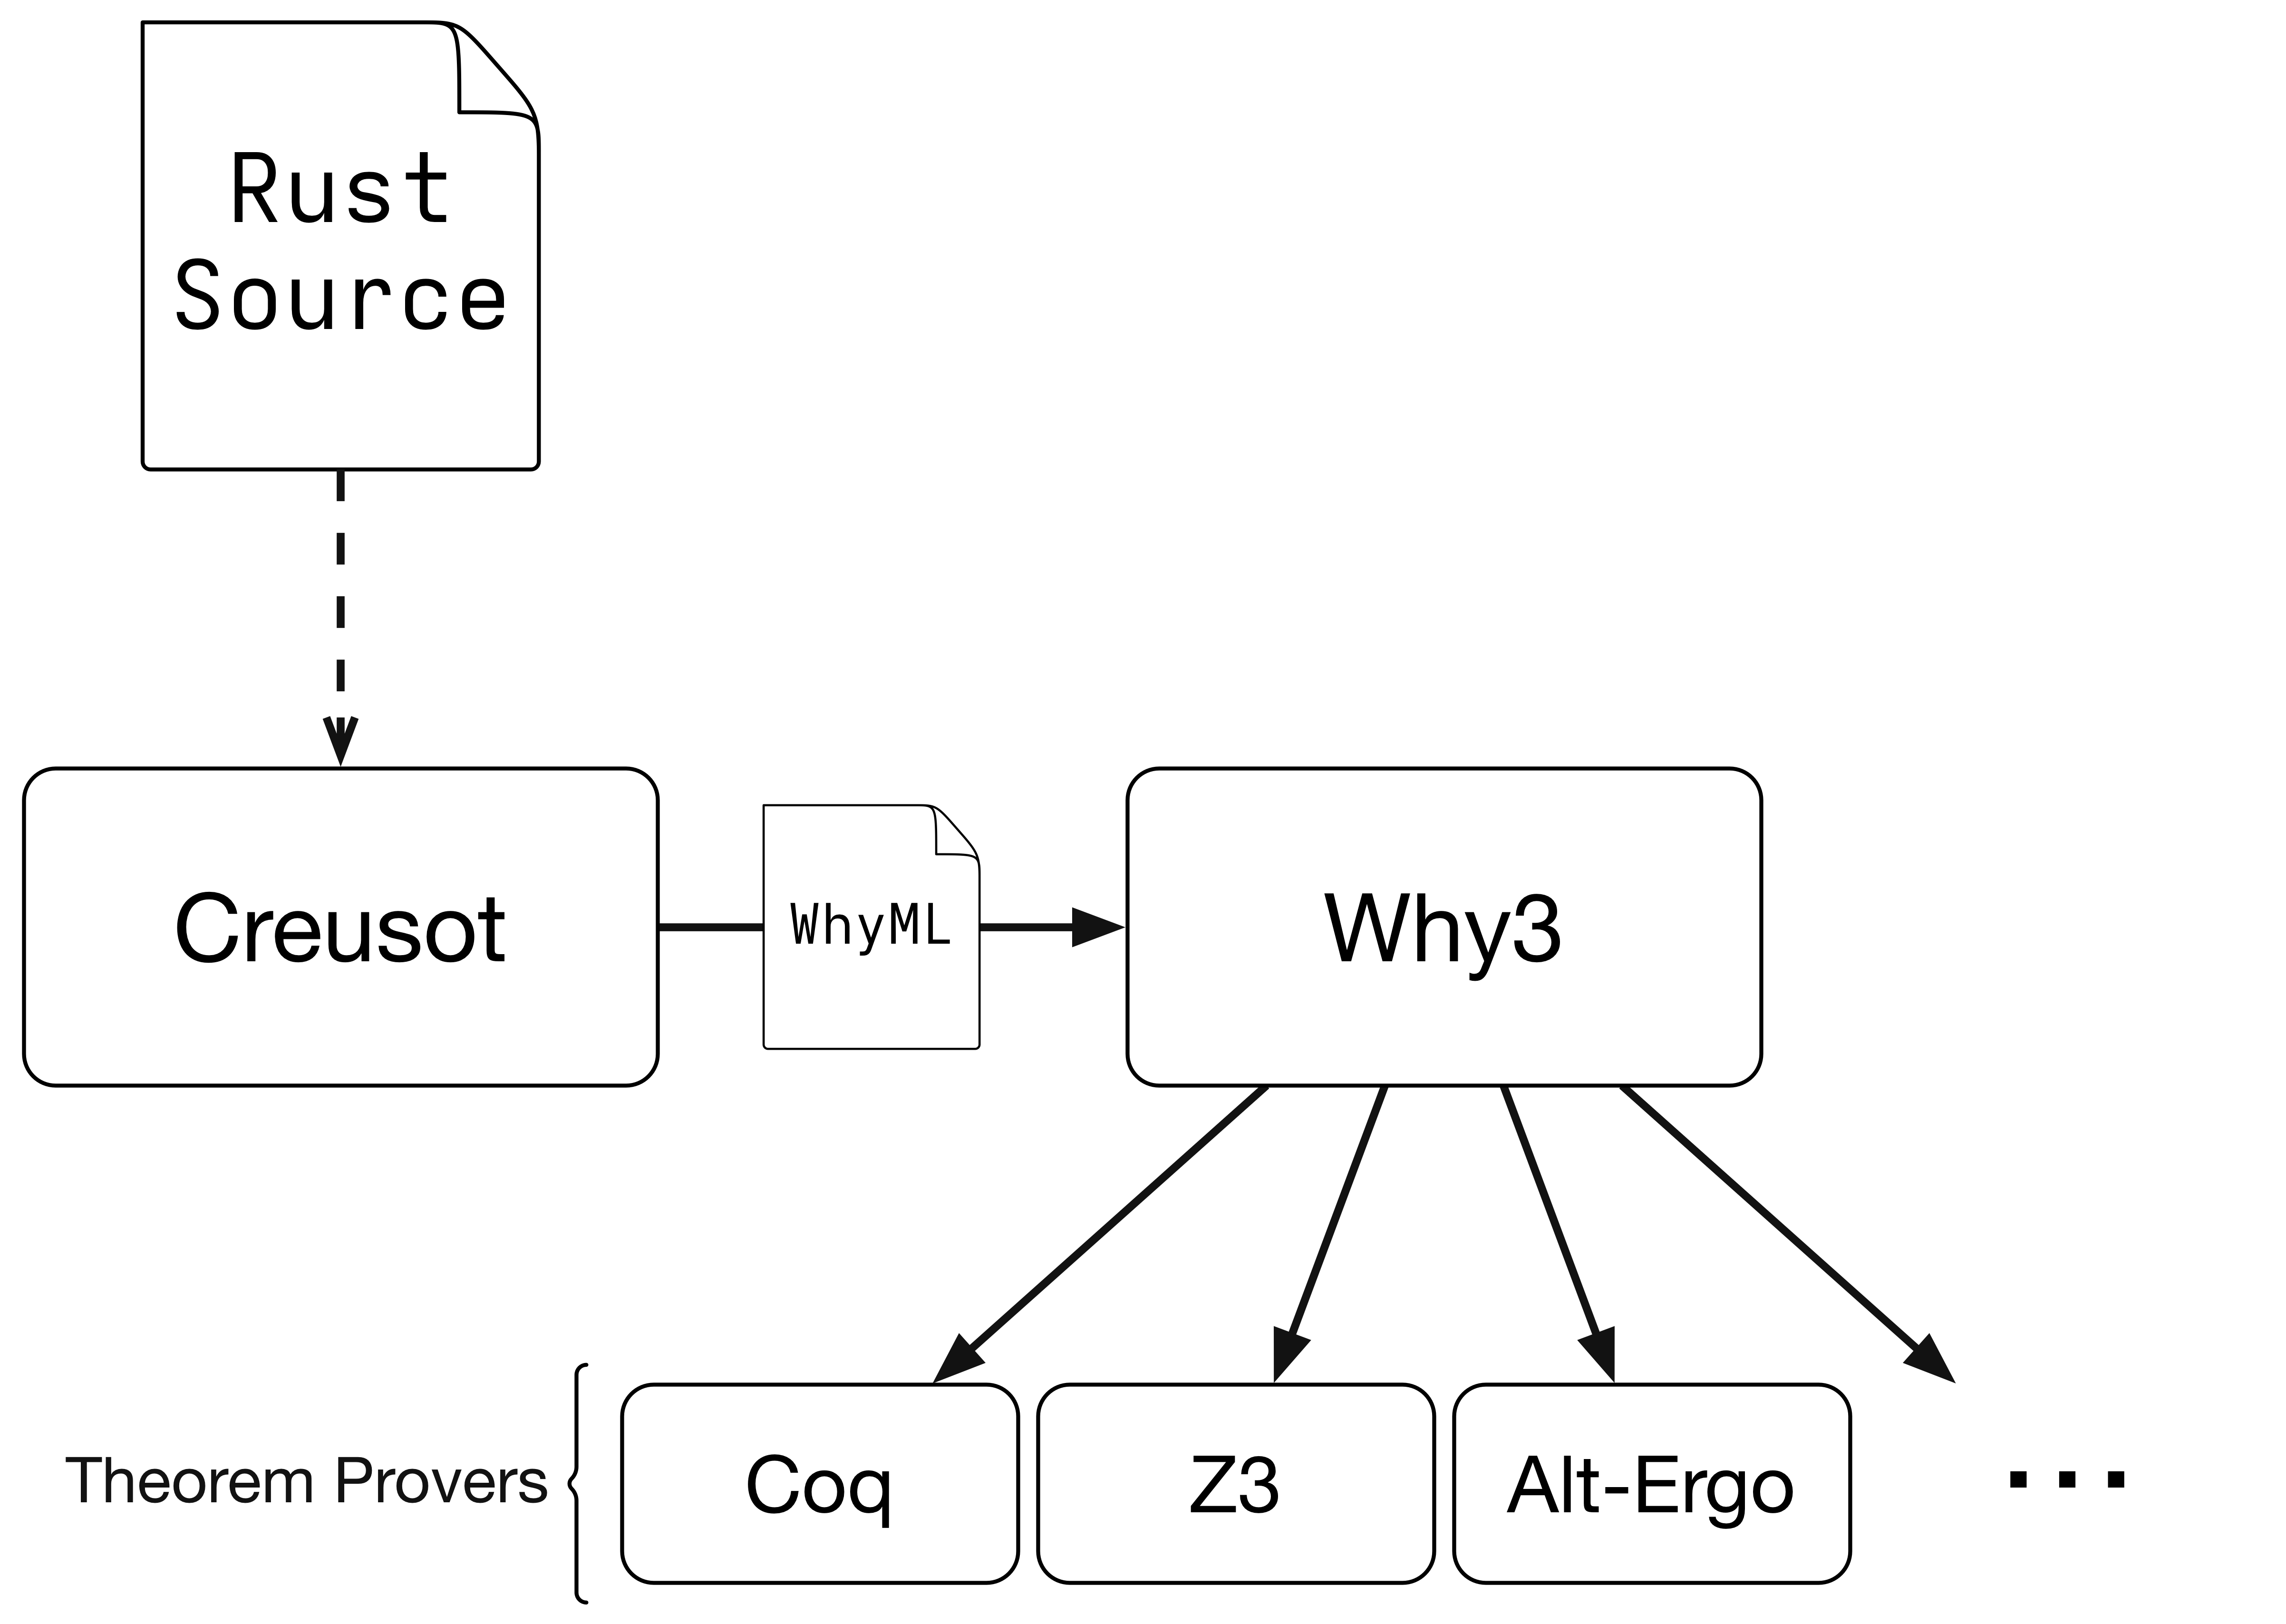
\includegraphics[width=0.5\textwidth]{creusot_why3_diagram}
\caption{How Creusot fits into the bigger picture}
\end{figure}

Why3 acts as a \emph{frontend} to various theorem provers---by targeting Why3, Creusot can take advantage of a wide variety of theorem provers with each of their unique strengths.
More about this in \ref{why-why3}.

% More on the tooling Creusot provides?

\section{Understanding Why3}
\label{why-why3}

Why3 describes itself as ``a platform for deductive program verification''\footnote{\url{https://why3.lri.fr/}}---instead of an interactive theorem prover like Coq or the like, Why3 is a layer above and focuses on automating the use of such provers.\cite{bobotWhy3ShepherdYour}
Why3 provides a language---called WhyML---that can be translated into languages a multitude of theorem provers can understand.
This is neat because we every prover has its strengths---Coq will be a better fit for certain proofs than fully-automated provers, whereas some provers will work without the laborious intervention that Coq requires.
Why3 allows us to have it all.

\subsection{WhyML}

WhyML has a well-specified structure\footnote{https://why3.lri.fr/doc/syntaxref.html}.
Let's take a brief look at WhyML to see how one would go about creating a simple specification.

Consider verifying a simple fact about arithmetic like $\forall x \in \mathbb{Z}, 2x = x + x$.
This is how we would write that in WhyML:

\begin{figure}[h]
\centering
\begin{verbatim}
module SumEquiv
  use int.Int

  goal SimpleThing: forall x:int. 2 * x = x + x
end
\end{verbatim}
\caption{SumEquiv: a very simple theorem showing that $\forall x \in \mathbb{Z}, 2x = x + x$}
\label{fig:sumequiv}
\end{figure}

This is an incredibly simple example; we will leave a full description of what the language can do to the specification\footnote{\url{https://why3.lri.fr/doc/syntaxref.html}}, but suffice it to say that WhyML has all of the language constructs that you would expect from a formal logic system.

% TODO: we should highlight some differences

\subsection{Discharging proofs}

The really exciting part of Why3 is how it can translate WhyML into input to various other theorem provers, interactive and automatic.
For example, we can ask the Alt-Ergo SMT solver to check that figure \ref{fig:sumequiv} holds, which it can do automatically.
There are several SMT solvers (e.g. Z3, CVC4, etc.) that Why3 can convert WhyML into and leverage.

% What are the strengths of one over another?

As nice as SMT solvers are, they are not able to do everything that interactive theorem provers can do.
Interactive provers---like Coq or Idris---allow a human to take control of the proof.
Fortunately, Why3 also supports using interactive provers to discharge individual proof steps.

We can ask Why3 to discharge the proof of \texttt{SimpleThing} with Coq.
Why3 opens the \texttt{coqide} with the following-filled for us:

\begin{verbatim}
(* This file is generated by Why3's Coq driver *)
(* Beware! Only edit allowed sections below    *)
Require Import BuiltIn.
Require BuiltIn.
Require int.Int.

(* Why3 goal *)
Theorem SimpleThing : forall (x:Numbers.BinNums.Z), ((2%Z * x)%Z = (x + x)%Z).
(* Why3 intros x. *)
intros x.

Qed.
\end{verbatim}

Now it is up to us to fill in the rest of the proof.

We have to use the ZArith module from the Coq standard library\footnote{\url{https://coq.inria.fr/library/Coq.ZArith.BinInt.html}} because Why3 works with integers, not naturals.
We can add this line after the \texttt{intros x.} to get Coq to accept the proof:

\begin{verbatim}
rewrite Z.add_diag. reflexivity.
\end{verbatim}

With that in place, we ask Why3 to ``replay obsolete proofs'' (in Why3 parlance) and it will run Coq, make sure that the intros and the theorem in the source still line up, and accept that theorem as proven if Coq succeeds.

Note that all proving \emph{must} go after the \texttt{(* Why3 intros x. *)} part and before the \texttt{Qed.} line.
This is so that Why3 can parse the source file and reliably rebuild the proof later on.

\section{How Rust enables Creusot}

% How does Creusot take advantage of Rust's unique type system & stuff to work?

% Why is it cool that it's using Rust?
% - macros
% - in-line documentation/verification markup
Creusot is a tool that, like similar tools in other languages, allows the user to annotate code with pre and post-conditions for deductive verification.
But, it uniquely gains several useful features from being used on the Rust programming language.
Rust is most widely known for being a programming language that allows for safe and efficient code because of its linear type system that can reason about memory safety at compile time.
It also has a powerful trait system for polymorphism and a sophisticated macro system.
This makes the language a perfect target for annotation-based verification.
Creusot makes use of macros, traits, and the ownership-borrowing model to do verification.

\subsection{Macros for annotations}
In Rust, macros can be used to work on the AST directly and give the user powerful metaprogramming capabilities.
Creusot makes specific use of macros that annotate statements and declarations in the program.
Within these annotations, we can use a prepositional logic language called Pearlite to write invariants.
\begin{verbatim}
#[requires(... precondition ...)]
#[ensures(... postcondition ...)]
fn my_function(i: u32) -> bool { ... }
\end{verbatim}

Here we can see that Creusot gives us some contract expressions in the form of annotation macros that let us specify the pre-conditions (using ``requires'') and post-conditions (using ``ensures'') of the function.
These expressions may refer to any of the arguments to the function as well as the final result.
With the Pearlite syntax, we may write prepositional logic with operators such as ``forall'', implies ("==>"), ``exists'', as well as the standard boolean operators.
Creusot also gives us the capability of writing Rust functions that can be used as custom predicates inside annotations.

These annotation macros can be read by the standard Rust compiler but are ignored.
However, the Creusot Rust compiler will read them as well as the Rust source code to generate WhyML code for verification.
This makes it so that Creusot annotations can show more semantic information than simple comments and allows verification to serve as clear in-line documentation.

\subsection{Ownership and borrowing of mutating pointers}
The biggest gains that Creusot gets from being on Rust is the ownership-borrowing system.
Most systems software is writing in languages like C/C++ which make frequent use of unbounded mutable pointers that can cause aliasing.
Aliasing wreaks havoc on verification software because two pointers may point to the same thing and mutate it throughout a program.
In Rust, every value is ``owned'' by an identifier. When that identifier goes out of scope, the value that the identifier refers to is dropped from memory.
You may, however, lend out a reference to the value, which in Rust is called ``borrowing''.
The identifier with a borrowed value may read the contents at the given location but it may not mutate it.
There is a special kind of borrow called a mutable borrow that does give the borrower mutable access to the value, however, the owner may only lend out one mutable reference at a time.
Given these properties of the language, Creusot is able to reason about mutating pointers through a technique called ``prophecies''.

In the Creusot paper, it gives an example of prophecies in action with a function called \texttt{gnome\_sort} which is a function that takes a mutable reference to a vector and sorts it in place.

\begin{verbatim}
#[ensures(sorted_range(@^v, 0, (@^v).len()))]
#[ensures((@^v).permutation_of(@*v))]
fn gnome_sort<T: Ord>(v: &mut Vec<T>) {
  let old_v = Ghost::record(&v);
  let mut i = 0;
  #[invariant(sorted_range(@*v, 0, @i))]
  #[invariant((@*v).permutation_of(@*@old_v))]
  while i < v.len() {
    if i == 0 || v[i - 1] <= v[i] {
    i += 1;
  } else {
    v.swap(i - 1, i);
    i -= 1;
  }
  }
}
\end{verbatim}

Creusot will look at the this mutable reference and create a ``prophecy'', which in WhyML is a record containing a current value and a final value.
The current value updates with every mutation to the value through the mutable reference but the final value is initialized to be a non-deterministic value that has yet to be resolved.
Fortunately, at the end of the function, when the mutable reference goes out of scope, the prophecy may safely resolve the final value to be the current value.
After which, the original owned value may be considered to be the final value of the mutable borrow.
This is all possible because there may only be one mutable borrow at a time and no aliasing.
So, whatever the borrowed value finishes as must be the new value of the owned variable.
In the sorting example, we can see that the annotations may refer to the current value of the reference (with the * operator) and also to the final value of the reference (with the \texttt{\^} operator).
Using an ``ensures'' clause, we can set a post-condition that the vector passed into the sorting function is sorted when the function exits.
(Here \texttt{sorted\_range} is a custom predicate).
You can see \texttt{\^v} which refers to the ``final'' value of v.
We can also make a post-condition that ensures that the final value of \texttt{v(\^v)} is a permutation of the current value of \texttt{v (*v)}.
Looking further down, we see that being able to refer to both the current value and final value of v is very useful when writing loop invariants.
Here, we are declaring a loop invariant that the current value of v (after each iteration) has a sorted subsequence from 0 to i.
Also, we declare that the the current value of v has remained a permutation of the original vector.
As we can see, Rust allows Creusot to not only reason about and verify mutating pointers but also gives user more powerful annotation capabilities.

\subsection{Creusot Traits}
Creusot also gains some conveniences from the Rust trait system.
Traits are similar to type classes in Haskell, and allow for polymorphism.
Traits define a set of functions that a datatype must implement.
Creusot defines two traits: Resolve and Model.
The Resolve trait lets the user specify what information can be gained when a value referred to inside an annotation is resolved.
This is what makes Creusot's annotations so semantically powerful and usable across many data types.
Another trait that helps with this is the Model trait. The Model trait simply allows users to treat a complex data structure in terms of a ``model'' which abstracts away the implementation details.
This is useful for referring to data structures inside annotations.

The Rust programming language, with it's strong static memory guarantees, trait system, and metaprogramming capabilities,
opened the door for tools like Creusot to make fine-grained static verification of mutating pointers not only possible, but also able to provide
semantically meaningful annotations for that verification on Rust code.

\section{Verification with Creusot}

Creusot works by installing a helper tool to run with Rust's \texttt{cargo} build and package manager.

\subsection{Example: verifying a simple function}

Consider the following Rust function:

\begin{verbatim}
#[requires(lo < hi)]
#[ensures(^lo < ^hi)]
fn palindrome_range(s: &[u8], lo: &mut usize, hi: &mut usize) {
    #[invariant(*lo < *hi)]
    #[invariant(*lo >= 0)]
    #[invariant(*hi < (s.deep_model()).len())]
    while *lo > 0 && *hi < s.len() - 1 && s[*lo - 1] == s[*hi + 1] {
        lo = lo - 1;
        hi = hi + 1;
    }
}
\end{verbatim}

This function takes a string, and and two integers \texttt{lo} and \texttt{hi} as mutable references.
It walks the string in opposite directions as long as \texttt{lo} and \texttt{hi} index into the same letter: in short, this walks palindromes inside of strings.

We have added some pre- and post-conditions to the function, namely that---as long as \texttt{lo} is less than \texttt{hi} at the beginning---their \emph{final values} will likewise be ordered.
We also need to specify some invariants on the \texttt{while} loop.

\section{Conclusion}

Rust makes building reliable software simple, and Why3 makes using automated theorem provers easy---what isn't there to like?
Unfortunately, the user experience with Creusot leaves a lot to be desired.
While we were working on this project we spent weeks just trying to get all of the Rust toolchains, libraries, etc. to line up just right so that we could compile Creusot.
Once we got Creusot compiled, we discovered that CreuSAT didn't work because it was built with an older version of Creusot.
Taylor was able to track down the version of Creusot that works with CreuSAT, and Ashton was able to plug everything together to get CreuSAT to verify.

However, the setup was brittle and easily slipped out of alignment.
Moreover, we found that many (all?) of the examples from the Creusot paper didn't work on this slightly out-of-date version of Creusot---they required a still older version of Creusot to run.
To top it all off, when we did find some examples that ran with the latest Creusot version, we soon ran into problems because the developers of Creusot shipped yet more breaking changes to Pearlite while we were in the process of trying to verify some code.

We think Creusot holds promise---Rust's popularity is exploding, and the lifetimes of Rust make analyzing it easy and robust.
Why3 is a really neat platform that brings together a lot of disparate tools and plays to their strengths.
However, the user experience of Creusot is just not there yet: there is \emph{no} up-to-date documentation that we were able to find, and the frequent breaks made using Creusot all but impossible.

To be fair, the authors of Creusot \emph{do} point out that this is unstable research software.\footnote{See the README of the Creusot\cite{denisCreusot2023} repository for this warning.}
If your work can tolerate frequent breakage, this might be a good option for you right now.
Neither of us would use this in its current form though---once things stabilize, however, Creusot will be a formidable addition to Rust's already substantial clout in the reliable software space.

\section{Resources}

\begin{description}
  \item[Creusot] \cite{denisCreusot2023} \cite{denisCreusotFoundryDeductive2022}

    Creusot is a formal verification tool written in Rust for verifying Rust programs.

  \item[CreuSAT] \cite{skotamCreuSAT2023}

    CreuSAT is a SAT solver verified with Creusot.
    CreuSAT pushes the boundaries of what Creusot can do.
    We were able to verify the source of CreuSAT after many tears and much lost sleep.
    Once we finally got the entire stack to compile, verification went off without a hitch thanks to some rather simple automatic verification strategies provided by CreuSAT.
    This showed off how Why3 can make verifying programs almost entirely automatic.

    CreuSAT shows that Creusot \emph{can} scale to significantly-sized projects.
    The UX and the documentation just aren't there for mainstream use, however.

  \item[Kani] \cite{Kani2023}

    From the README: Kani is particularly useful for verifying unsafe code in
    Rust, where many of the language's usual guarantees are no longer checked by
    the compiler.

    We ran out of time before we were able to evaluate Kani for this project.
    It does seem like an intriguing piece of software however.

\end{description}

\clearpage
\printbibliography

\end{document}

% Local Variables:
% jinx-local-words: "CreuSAT Creusot's Kani Pearlite WhyML creusot"
% End:
